\chapter{An Overview of Numerical Optimization}
\label{cha:overviewpart1}
In this chapter, we aim to provide readers with an overview of numerical optimization. We begin with the theory of optimization (Section~\ref{sec:theory}), from the existence of optimizers, to the optimality conditions for both unconstrained and constrained problems with duality. As the theoretical background of optimization, this field provides a solid solution for the algorithm. 
\par We then formally define the optimization of unconstrained and constrained problems in Section~\ref{sec:consopt} and describe the general regular solution for these problems based on the gradient calculation. 
\par Next, we discuss briefly the bi-level optimization, which is a lower-level optimization problem embedded within an upper-level problem sharing the same variables. (Section~\ref{sec:bilevel}). Finally, we give a summary of the numerical optimization in constrained problems in Section~\ref{sec:2summary}.




\section{Theory of Optimization}
\label{sec:theory}
\subsection{Existence of Optimizers}
In optimization, a basic question is to determine the existence of a global minimizer for a given function $f$. There are several sufficient conditions on $f$ to guarantee the existence, and the optimizer falls in the feasible set of solutions. For a feasible set, some related definitions are following: 
\begin{defn}
    A subset $\Omega \in \mathbb{R}^n$ is called
    \begin{itemize}
        \item \emph{bounded} if there is a constant $R > 0$ such that $\|x\| \leq R$ for all $x \in \Omega$
        \item \emph{closed} if the limit point of any convergent sequence in $\Omega$ always lies in $\Omega$
        \item \emph{compact} if any sequence $\left\{x_{k}\right\}$ in $\Omega$ contains a subsequence that converges to a point in $\Omega$
    \end{itemize}
\end{defn}
\par The following result gives a characterization of compact sets in $\mathbb{R}$. When we find the minimum or maximum solution for the problem, there exists a lower bound or upper bound but not necessarily an optimal solution. Therefore, we have some additional requirements. 
\par Firstly, we give the definition of compact sets in Lemma~\ref{lemma:bw}. ~\citep{OG:17} gives a brief proof.
\begin{lemma}[Bolzano-Weierstrass theorem]
    \label{lemma:bw}
    A subset $\Omega$ in $\mathbb{R}^n$ is \emph{compact} if and only if it is bounded and closed.
\end{lemma}
\par We also assume that the function $f$ is continuous and "$+\infty$ at infinity". More precisely, $f(x) \rightarrow+\infty$ if $|x| \rightarrow+\infty$. Such a function is called \emph{inf-compact} or \emph{coercive}.~\citep{JS:06} Then the problem can be restricted to a bounded set and existence of a global minimum $x^{*}$ is guaranteed: a continuous function has a minimum on a compact set. This theorem is defined as follows and the proof is given in Appendix~\ref{appendix:trm23}.
\begin{thm}~\citep{JS:06}
    \label{thm:23}
    If $f$ is a continuous function defined on a compact set $\Omega$ in $\mathbb{R}$, then $f$ has a global minimizer $x^{*}$ on $\Omega$ i.e. there exists $x^{*} \in \Omega$ such that $f\left(x^{*}\right) \leq f(x)$ for all $x \in \Omega$
\end{thm}
More general, based on the definition of coercive function $f$, we can give following theorem. Proof is given in Appendix~\ref{appendix:trm24}.
\begin{thm}~\citep{JS:06}
    \label{thm:24}
    If $f: \mathbb{R}^{n} \rightarrow \mathbb{R}$ is a continuous coercive function, then $f$ has at least one global minimizer.
\end{thm}
Theorem~\ref{thm:24} requires the continuity of $f$ which is somewhat restrictive for applications. However, we can replace it by the lower semi-continuity of $f$ which is a rather weaker condition. 
\begin{defn}
    Let $f: \mathbb{R}^{n} \rightarrow \mathbb{R} \cup\{\pm \infty\}$. Then $f$ is called \emph{lower semi-continuous} at a point $x_0 \in \mathbb{R}^n$ if for any sequence $f\left(x_{k}\right)$ converging to $x_0$ here holds $f\left(x_{0}\right) \leq \lim _{k \rightarrow \infty} f\left(x_{k}\right)$. $f$ is called \emph{lower semi-continuous} if $f$ is lower semi-continuous at every point.
\end{defn}
Recall our assumptions on function $f$, it is a continuous function, which is always lower semi-continuous. However, lower semi-continuous functions are not necessarily continuous. For instance, a binary function equals to 0 when $x \leq 0$ and equals to 1 when $x > 0$ is not continuous at $x_0 = 0$. However, since it is greater than 0 for all $x$ and $f(0) = 0$, we have $f(0)=0 \leq \liminf _{x \rightarrow 0} f(x)$ and it is lower semi-continuous at $x_0 = 0$.
\par The theorem of the existence of the optimizer of lower semi-continuous function is given as follows and the proof is given in Appendix~\ref{appendix:thm25}
\begin{thm}~\citep{JS:06}
    \label{thm:25}
    Let $f: \mathbb{R}^{n} \rightarrow \mathbb{R}$ be a lower semi-continuous function. If $f$ has a nonempty, compact sublevel set $D:=\left\{x \in \mathbb{R}^{n}: f(x) \leq \alpha\right\}$, then $f$ achieves a global minimizer on $\mathbb{R}$
\end{thm}
Also, we introduce the definition of convex function and convex set which are important in regular optimization problems.
\begin{defn}
    A function $f$ is convex when 
    $$
        f(\alpha x+(1-\alpha) y) \leq \alpha f(x)+(1-\alpha) f(y) \quad \textrm{for all } x, y, \textrm{ and } \alpha \in ]0,1[
    $$
    A set $C \subset \mathbb{R}^n$ is convex when 
    $$
    \alpha x+(1-\alpha) y \in C \quad \textrm { for all } x, y \textrm { in } C, \textrm{ and } \alpha \in ] 0,1[
    $$
\end{defn}
The problem we are going to discuss in this part is convex and regular, which means its gradient can be computed and the solution exists. However, although the existence of the optimizer is sufficient, for different problems, the optimality conditions are different. In the next two sections, we will give necessary and sufficient conditions for both unconstrained and constrained problems.

\subsection{Optimality Conditions for Unconstrained Problems}
Firstly, we consider the unconstrained minimization problem
$$
\min _{\mathbf{x} \in \mathbb{R}^{n}} f(x),
$$
where $f$ is given function on $\mathbb{R}^n$. 
\par In order to determine the minimizer, it is important to understand what can happen at a minimizer, and at what condition a point must be a minimizer. Now we have to recognize the optimum point. There are two necessary conditions and one sufficient condition given below~\citep{JS:06}. The proof is given in Appendix~\ref{appendix:thm28}.
\begin{thm}{Necessary and Sufficient Conditions.}
    \label{thm28}
    Let $f:\Omega \rightarrow \mathbb{R}$ be a funcion defined on a set $\Omega \subset \mathbb{R}^n$ and let $x^*$ be an interior point of $\Omega$ that is a local minimizer of $f$. \\
    Necessary conditions:
    \begin{itemize}
        \item (NC1) If $f$ is differentiable at $x^*$, then $x^*$ is a critical point of $f$, i.e. $\nabla f\left(x^{*}\right)=0$.
        \item (NC2) If $f$ is twice continuous differentiable on $\Omega$, then the Hessian $\nabla^2 f\left(x^{*}\right)$ is positive semidefinite.
    \end{itemize}
    Sufficient condition (SC1): if $x^*$ is such that $\nabla f\left(x^{*}\right)=0$ and $\nabla^2 f\left(x^{*}\right)$ is positive definite, then $x^*$ is a local minimum. (i.e. $f(x) \geq f(x^*)$ for $x$ close to $x^*$)
\end{thm}
\par Any point satisfying (NC1) as the minimizer of $f$ is called a \emph{critical} or \emph{stationary} point of $f$. In the objective function $f$ is convex, (NC1) is also the sufficient condition for the global minimum of the solution. 
\par Let us see an example of unconstrained minimization problem. Supposed we have to determine the minimization of function
$$
f(x, y)=x^{4}-4 x y+y^{4}
$$
From the definition of function $f$, it is clear that $f$ is continuous. Then we can expand $f$ by writing
$$
f(x, y)=\left(x^{4}+y^{4}\right)\left(1-\frac{4 x y}{x^{4}+y^{4}}\right)
$$
we can see $f$ is coercive. Also, we give the plotting graph of function $f$ in Figure~\ref{fig:unconseg}. Therefore $f$ has global minimizers which are critical points. Now according to (NC1), we can find the global minimizer through solving the derivative of $f$ equaling to zero:
$$
0=\nabla f(x, y)=\left(\begin{array}{c}4 x^{3}-4 y \\ -4 x+4 y^{3}\end{array}\right)
$$
\par Thus, $y = x^3$ and $x = y^3$. Consequently $y = y^9$, i.e.
$$
0=y-y^{9}=y\left(1-y^{8}\right)=y\left(1-y^{4}\right)\left(1+y^{4}\right)=y(1-y)(1+y)\left(1+y^{2}\right)\left(1+y^{4}\right)
$$
\par This implies $y = 0, 1, -1$. Thus $f$ has three critical points $(0,0), (1,1), (-1,-1)$. Then we can evaluate $f$ as these points since they may be local minimizer:
$$
f(0,0)=0, \quad f(1,1)=-2, \quad f(-1,-1)=-2
$$
\par It achieves the same global minimum value on $(1, 1)$ and $(-1, -1)$. Therefore, they are both global minimizers of $f$. 
\begin{figure}[t]
\label{fig:unconseg}
\centering
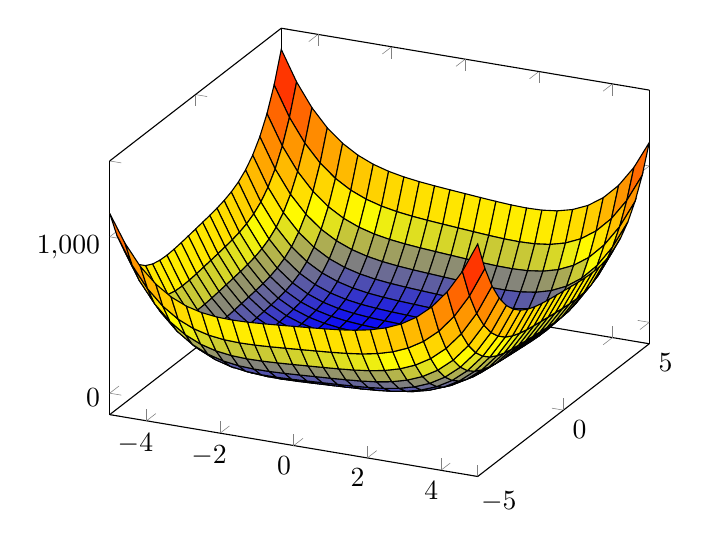
\begin{tikzpicture}
    \centering
    \begin{axis}
    \addplot3 [surf,shader=flat,draw=black] {x^4-4*x*y+y^4};
    \end{axis}
\end{tikzpicture}
\caption{Function Graph of $f(x, y)=x^{4}-4 x y+y^{4}$}
\end{figure}
\par From this example, we verify that through (NC1), we can find the global minimizer. However, not all continuous functions with critical points have any maximizer or minimizer. If the function goes to infinity along its axes or a line, it does not have any maximizer or minimizer although it has a critical point. The condition of the minimizer as the critical point is that the function $f$ should be a convex function with continuous first partial derivatives.
\par Let us move to the sufficient condition (SC1). The result obtained under this theorem is best possible for general functions. Specifically, for a convex function $f$ is defined on a convex set $\Omega \subset \mathbb{R}^n$, any local minimizer of f is also a global minimizer. Moreover, if a function $f$ is strictly convex, it has at most one global minimizer. 

\subsection{Optimality Conditions for Constrained Problems}
A general formulation for constrained optimization problems is as follows: 
$$
\begin{array}{l}\textrm { minimize } f(x) \\ \textrm { subject to }\left\{\begin{array}{ll}c_{i}(x)=0 & \textrm { for } i=1, \cdots, m_{e}, \\ c_{i}(x) \leq 0 & \textrm { for } i=m_{e}+1, \cdots, m\end{array}\right.\end{array}
$$
where $f$ and $c_i$ are smooth real-valued functions on $\mathbb{R}^n$, and $m_e$ and $m$ are nonnegative integers with $m_e < m$. We set 
$$
\mathbb{E}:=\left\{1, \cdots, m_{e}\right\} \quad \textrm { and } \quad \mathbb{I}:=\left\{m_{e}+1, \cdots, m\right\}
$$
as index sets of equality constraints and inequality constraints, respectively. Here, $f$ is so-called the objective function, and $c_i, i \in \mathbb{E} \textrm{ and } \mathbb{I}$ are equality constraints and inequality constraints respectively. 




\subsection{Duality}


\section{Unconstrained and Constrained Optimization}
\label{sec:consopt}
\subsection{Unconstrained Optimization}
\subsection{Equality Constrained Optimization}
\subsection{Inequality Constrained Optimization}

\section{Bi-level Optimization}
\label{sec:bilevel}



\section{Summary}
\label{sec:2summary}
Summary what you discussed in this chapter, and mention the story in next
chapter. Readers should roughly understand what your thesis takes about by only reading
words at the beginning and the end (Summary) of each chapter.



